\documentclass{beamer}
\usepackage{graphicx}

% Naslovnica
\title{Napredna računališka orodja, 1. domača naloga}
\author{Luka Ogrinc}
\institute{Univerza v Ljubljani, Fakulteta za strojništvo}
\date{23. 10. 2023}

% Dodatek za logotip FS
\logo{
\includegraphics[height=1cm]{fs-logo.jpg}}

% Začetek dokumenta
\begin{document}

\frame{\titlepage}

% Kazalo
\begin{frame}
\frametitle{Kazalo}
\tableofcontents
\end{frame}

% Prva sekcija
\section{Uvod}

\begin{frame}
\frametitle{Uvod}
Za 1. domačo nalogo smo v Matlab jeziku in programskem okolju z metodo Monte Carlo izračunali približek številu $\pi$.
\end{frame}

% Slika s podnapisom

\section{Monte Carlo metoda}

\begin{frame}
\frametitle{Monte Carlo metoda}
\begin{figure}
\centering
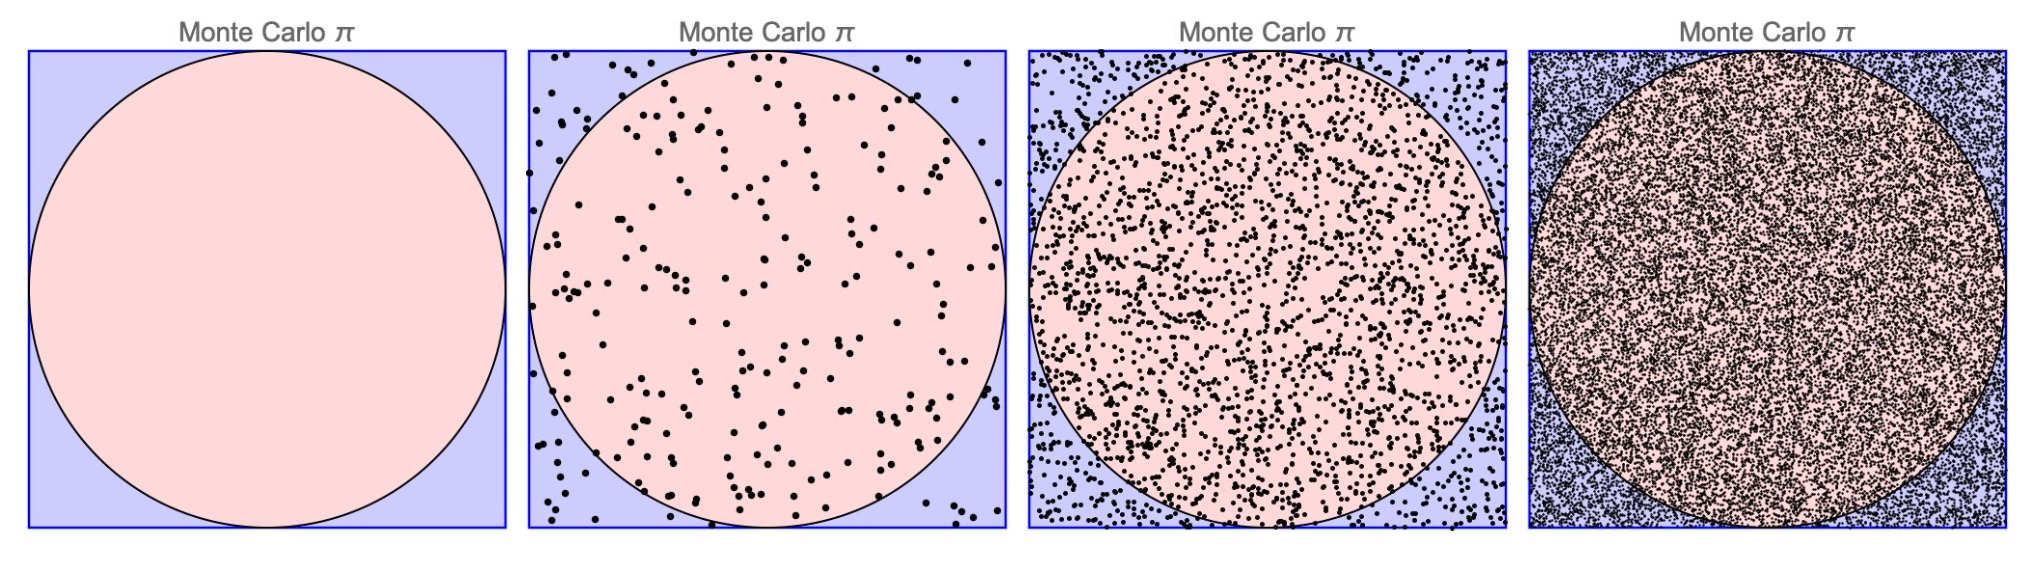
\includegraphics[width=1\textwidth]{slika.jpg}
\caption{Prikaz Monte Carlo metode, kjer se vidi generiranje naključnih točk.}
\end{figure}
\end{frame}

% Tretja sekcija
\section{Rezultati}

\begin{frame}
\frametitle{Rezultati}
Na koncu smo ustvarili datoteke:
\begin{itemize}
  \item calc\_pi.m,
  \pause
  \item mcc\_pi.m in
  \pause
  \item plot\_random\_points.m.
\end{itemize}
\end{frame}


\end{document}
